\documentclass[11pt, A4paper,norsk]{article}
\usepackage[utf8]{inputenc}
\usepackage[T1]{fontenc}
\usepackage{babel}
\usepackage{amsmath}
\usepackage{amsfonts}
\usepackage{amsthm}
\usepackage{amssymb}
\usepackage[colorlinks]{hyperref}
\usepackage{listings}
\usepackage{color}
\usepackage{hyperref}
\usepackage{graphicx}
\usepackage{cite}
\usepackage{textcomp}
\usepackage{float}

\definecolor{dkgreen}{rgb}{0,0.6,0}
\definecolor{gray}{rgb}{0.5,0.5,0.5}
\definecolor{daynineyellow}{rgb}{1.0,0.655,0.102}
\definecolor{url}{rgb}{0.1,0.1,0.4}

\lstset{frame=tb,
	language=Python,
	aboveskip=3mm,
	belowskip=3mm,
	showstringspaces=false,
	columns=flexible,
	basicstyle={\small\ttfamily},
	numbers=none,
	numberstyle=\tiny\color{gray},
	keywordstyle=\color{blue},
	commentstyle=\color{daynineyellow},
	stringstyle=\color{dkgreen},
	breaklines=true,
	breakatwhitespace=true,
	tabsize=3
}

\lstset{inputpath="C:/Users/Torstein/Documents/UiO/Fys2140/Python programmer"}
\graphicspath{{C:/Users/Torstein/Documents/UiO/Fys2140/"Python programmer"/}}
\hypersetup{colorlinks, urlcolor=url}

\author{Kandidatnummer: 15159}
\title{Svar på Hjemmeeksamen i Fys2140}



%\lstinputlisting{Filnavn! type kodefil}
%\includegraphics[width=12.6cm,height=8cm]{Filnavn! type png}



\begin{document}
\maketitle
	\begin{center}
\includegraphics[scale=1]{{C:/Users/Torstein/Documents/UiO/uio.jpeg}}
	\end{center}
\clearpage
	\begin{center}
\Large \textbf{Oppgaver}
	\end{center}









		\paragraph{1.a}
			\subparagraph{1)}
				\begin{flushleft}
Comptons formel er
$$\lambda_C = \frac{h}{m c}$$
Her er $\lambda_C$ Comptonbølgelengden, $h$ er Plancks konstant, $m$ er massen til den eventuelle partikkelen du ønsker å finne Comptonbølgelengden til og $c$ er lysets hastighet i vakum.
				\end{flushleft}
				\begin{figure}[H]
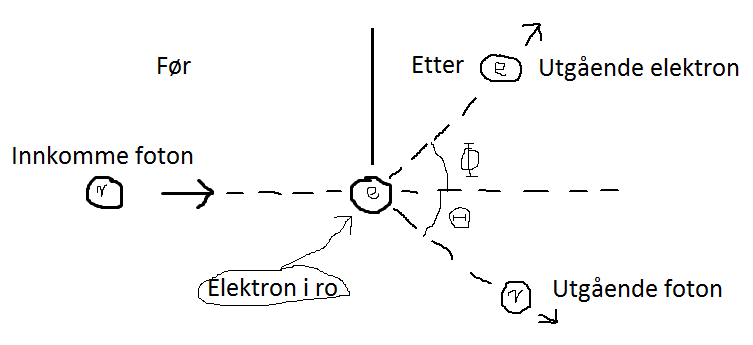
\includegraphics[width=13cm,height=9cm]{Comptonspredning.png}
\caption{Prinsippskisse av fotonspredning, sånn som i Comptons forsøk}
				\end{figure}
				\begin{flushleft}
Figuren viser et foton som kolliderer med et elektron, som er i ro, og overfører deler av bevegelsesmengden sin til elektronet. Bevegelsesmengden er bevart så det er en sammenheng mellom vinklene $\theta$, $\phi$, bevegelsesmengden til elektronet og fotonet.
				\end{flushleft}
				\begin{gather*}
\text{Regner ut Compton bølgelengden ved hjelp av Comptons formel} \\
\lambda_C = \frac{h}{m_e c} = \frac{6.626 \cdot 10^{-34} \text{Js}}{(9.109 \cdot 10^{-31} \text{kg}) \cdot (2.998 \cdot 10^{8} \text{m}/\text{s})} \\
\lambda_C \approx 2.43 \cdot 10^{-12} m = 2.43 \cdot 10^{-2} \text{Å}
				\end{gather*}






			\subparagraph{2)}
				\begin{gather*}
\text{Antar det er meningen her at vi skal regne ut for hvilken vinkel han burde ha} \\
\text{målt $\lambda' = 0.0749 \text{nm}$, og ikke tippe ut i fra Figur $1$ hva vinkelen skal være.} \\
\text{Fra likning (2.32) i kompendiet har vi at} \\
\Delta \lambda = (\lambda' - \lambda_0) = \frac{h}{m_e c} (1 - \cos(\theta)) \\
1 - \frac{\lambda' - \lambda_0}{\lambda_C} = \cos(\theta) \\
\cos(\theta) = 1 - \frac{0.0749 \text{nm} - 0.0709 \text{nm}}{2.43 \cdot 10^{-3} \text{nm}} \\
\theta \approx 130.2^{\circ} \\
\text{Hvis det er meningen at jeg skal gjette hvilken vinkel han målte ut i} \\
\text{fra figuren ville jeg fra dette gjettet på $135^{\circ}$}
				\end{gather*}









			\subparagraph{3)}
				\begin{flushleft}
Grunnen til at A. H. Compton fikk en topp som ser ut som den ligger ved $\lambda_0$ er at noen av elektronene, som fotonene han sender inn reagerer med, vil være såpass sterkt bundet til atomet at vi er nødt til å se på kollisjonen som, ikke mellom foton og elektron, men foton og atom. Da vil massen til atomet gjøre at Comptonbølgelengden blir veldig mye større enn $\Delta \lambda$ og vi vil ikke kunne se forskjellen mellom $\lambda_0$ og denne bølgelengden. \\
Det er litt den samme grunnen for hvorfor Compton ikke brukte synlig lys. Hadde han brukt synlig lys ville den største mulige endringen $\Delta \lambda$ være så liten at vi knapt nok kan se den. Dette på grunn av at bølgelengdene til synlig lys er så mye større enn endringene i bølgelengdene.
				\end{flushleft}
			








		\paragraph{1.b}
			\subparagraph{1)}
				\begin{flushleft}
Hvis den gjennomsnittlige energien til termiske nøytroner er gitt ved $\langle E \rangle = \frac{3}{2} k_B T$ der $k_B = 8.617 \cdot 10^{-5} \text{eV}/\text{K}$ er Boltzmanns konstant og $T = 25^{\circ}\text{C} = ( 25 + 273.15 )^{\circ} K = 298.15^{\circ} K$ er temperaturen til omgivelsene. Finner et tall for nøytronets gjennomsnittlige energi.
$$\langle E \rangle = \frac{3}{2} k_B T = \frac{3}{2} \cdot 8.617 \cdot 10^{-5} \text{eV}/\text{K} \cdot 298.15 K = 3.854 \cdot 10^{- 2} \text{eV}$$
Deretter finner vi gjennomsnittlig bevegelsesmengde utrykket $\langle p \rangle = \frac{E}{c}$
$$\langle p \rangle = \frac{\langle E \rangle}{c} = \frac{3.854 \cdot 10^{- 2} \text{eV}}{2.998 \cdot 10^{8} \text{m} / \text{s}} = 1.286 \cdot 10^{-10} \frac{\text{eV}}{\text{m} / \text{s}}$$
til slutt skal bølgelengden til en partikkel være gitt ved $p = \frac{h}{\lambda}$ så da blir gjennomsnitts bølgelengden
$$\langle \lambda \rangle = \frac{h}{\langle p \rangle} = \frac{h c}{\langle p \rangle c} = \frac{1240 \text{eV} \text{nm}}{3.854 \cdot 10^{- 2} \text{eV}} = 32170 \text{nm} = 32.17 \mu \text{m}$$
				\end{flushleft}










			\subparagraph{2)}
				\begin{flushleft}
Setter opp Braggs lov på formen for å finne vinkelen $\theta$
$$\theta = \arcsin \left( \frac{m \lambda}{2 d} \right)$$
det som gir den høyeste intensiteten er hvis $m = 1$. Da får vi at vinkelen blir
$$\theta = \arcsin\left( \frac{\lambda}{2 d} \right) = \arcsin\left( \frac{1.85 \text{Å}}{2 \cdot 2.82 \text{Å}} \right) = 0.334 = 19.15^{\circ}$$
Antar at vi må bruke $m = 1$, altså når bølgene har maksimal itensitet, for at vi skal kunne skille bølgene fra hverandre.
Hvis $\frac{|\Delta \lambda|}{\lambda} = \frac{|\Delta \lambda|}{1.85 \text{Å}} = 0.1 \Rightarrow |\lambda' - \lambda| = 0.1 \cdot 1.85 \text{Å} = 0.185 \text{Å} \Rightarrow \lambda' = 1.85 \text{Å} \pm 0.185 \text{Å} = 2.035 \text{Å} \wedge 1.665 \text{Å}$ så kan vi bruke Braggs lov til å finne hvilket vinkelspenn vi trenger for å finne disse bølgelengdene.
$$\theta = \arcsin\left( \frac{\lambda}{2 d} \right) = \arcsin\left( \frac{2.035 \text{Å}}{2 \cdot 2.82 \text{Å}} \right) = 0.3691 = 21.15^{\circ}$$
$$\theta = \arcsin\left( \frac{\lambda}{2 d} \right) = \arcsin\left( \frac{1.665 \text{Å}}{2 \cdot 2.82 \text{Å}} \right) = 0.2997 = 17.17^{\circ}$$
Altså blir vinkelområdet $\theta \in [2.997, 3.691] \vee [17.17^{\circ}, 21.15^{\circ}]$
				\end{flushleft}









		\paragraph{2.}
			\subparagraph{a)}
				\begin{flushleft}
Normerer bølgen $\Psi(x, 0) = A e^{- \frac{(x - x_0)^2}{4a^2}} e^{ikx}$
				\end{flushleft}
				\begin{gather*}
\int_{- \infty}^{\infty} |\Psi(x, 0)|^2 dx = \int_{- \infty}^{\infty} A^2 e^{- \frac{2 (x - x_0)^2}{4a^2}} e^{ikx} e^{- ikx} dx = A^2 \int_{- \infty}^{\infty} e^{- \frac{(x - x_0)^2}{2a^2}} dx \\
A^2 \int_{- \infty}^{\infty} e^{- \frac{x^2 - 2 x_0 x + x_0^2}{2a^2}} dx = A^2 \sqrt{\frac{\pi}{\frac{1}{2a^2}}} e^{\frac{\left( \frac{- x_0}{2 a^2} \right)^2 - \frac{1}{2a^2} \frac{x_0^2}{2a^2}}{\frac{1}{2a^2}}} \\
\int_{- \infty}^{\infty} |\Psi(x, 0)|^2 dx = A^2 \sqrt{2 \pi a^2} e^{\frac{\left( - x_0 \right)^2 - x_0^2}{2a^2}} = 1 \\
A = \frac{1}{\sqrt[4]{2 \pi a^2}} e^{- \frac{x_0^2 - x_0^2}{4a^2}} = \frac{1}{\sqrt[4]{2 \pi a^2}} \\
\Psi(x, 0) = \frac{1}{\sqrt[4]{2 \pi a^2}} e^{- \frac{(x - x_0)^2}{4a^2}} e^{ikx}
				\end{gather*}
				\begin{flushleft}
Plottet absoluttverdien av bølgefunksjonen i annen. Den blir en gaussisk bølge funksjon som har midpunkt i $5 \text{fm}$.
				\end{flushleft}
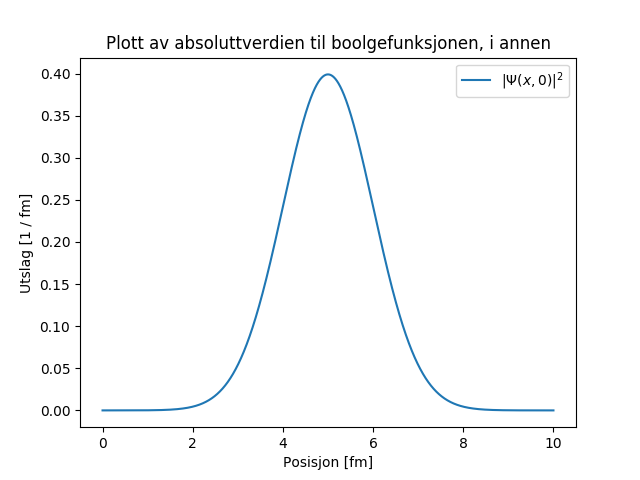
\includegraphics[width=12.6cm, height=9cm]{Figur_06.png}
\lstinputlisting{Hjemmeeksamen_2a.py}
				\begin{flushleft}
Siden vi kan anta at partikkelen ikke befinner seg i noe potensial så vil all energi være kinetisk energi og vi kan finne gjennomsnittsenergien ved hjelp av forventningsenergien til $p^2$.
				\end{flushleft}
				\begin{gather*}
\langle E_k \rangle = \frac{\langle p^2 \rangle}{2m} \\
\langle p^2 \rangle = \int_{- \infty}^{\infty} \Psi^{*} \left( - \hbar^2 \frac{d^2}{dx^2} \right) \Psi dx \\
\langle p^2 \rangle = \int_{- \infty}^{\infty} \left( \frac{1}{\sqrt[4]{2 \pi a^2}} e^{- \frac{(x - x_0)^2}{4a^2}} e^{- ikx} \right) \left( - \hbar^2 \frac{d^2}{dx^2} \right) \left( \frac{1}{\sqrt[4]{2 \pi a^2}} e^{- \frac{(x - x_0)^2}{4a^2}} e^{ikx} \right) dx \\
- \frac{\hbar^2}{\sqrt{2 \pi a^2}} \int_{- \infty}^{\infty} e^{- \frac{(x - x_0)^2}{4a^2}} e^{- ikx} \left( \frac{(x - x_0)^2}{4a^4} - \frac{ik (x - x_0) + 1}{2a^2} - k^2 \right) e^{- \frac{(x - x_0)^2}{4a^2} + ikx} dx \\
- \frac{\hbar^2}{\sqrt{2 \pi a^2}} \int_{- \infty}^{\infty} e^{- \frac{(x - x_0)^2}{2a^2}} \left( \frac{(x - x_0)^2}{4a^4} - \frac{ik (x - x_0) + 1}{2a^2} - k^2 \right) dx \\
\text{Kunne løst dette med Rottmann, men løser integralet på nett og får $\frac{\sqrt{{\pi}}\left( 4a^2k^2+1 \right)}{2^\frac{3}{2} a}$} \\
\langle p^2 \rangle = \frac{\hbar^2}{\sqrt{2 \pi a^2}} \frac{\sqrt{{\pi}}\left( 4 a^2 k^2 + 1 \right)}{2^\frac{3}{2} a} = \frac{\hbar^2}{4 a^2} \left( 4 a^2 k^2 + 1 \right) \\
\langle E_k \rangle = \frac{\hbar^2}{8 m a^2} \left( 4 a^2 k^2 + 1 \right)
				\end{gather*}









			\subparagraph{b)}
				\begin{flushleft}
Skisserer potensialet i paint <3 \\
Det er en graf som er null, uten om mellom $x_1$ og $x_2$ der den er lik $V_0$.
				\end{flushleft}
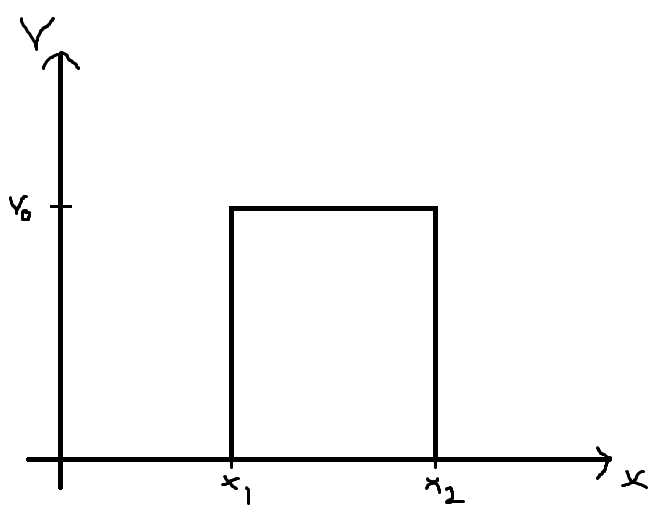
\includegraphics[width=13cm, height=9cm]{Potensial.png}
				\begin{flushleft}
Setter opp TUSL
$$- \frac{\hbar^2}{2m} \frac{d^2 \psi}{dx^2} + V \psi = E \psi$$
For $0 \leq x < x_1$ og $x_2 \leq x$ blir potensialet $0$ og vi får at TUSL blir
$$- \frac{\hbar^2}{2m} \frac{d^2 \psi}{dx^2} = E \psi \Rightarrow \frac{d^2 \psi}{dx^2} = - \frac{2 m E}{\hbar^2} \psi$$
De generelle løsningene for dette blir
$$\psi = Ae^{i k x} + Be^{- i k x} \wedge \psi = Fe^{i k x} + Ge^{- i k x}$$
der $k = \frac{\sqrt{2 m E}}{\hbar}$. $G$-leddet kan fjernes fordi det antas at det ikke kommer noen partikkel inn fra høyre, og vi får
$$\psi = Fe^{i k x}$$
Når $x_1 \leq x \leq x_2$ så er potensialet $V_0$ og vi får TUSL som
$$- \frac{\hbar^2}{2m} \frac{d^2 \psi}{dx^2} + V_0 \psi = E \psi \Rightarrow \frac{d^2 \psi}{dx^2} = - \frac{2 m (E - V_0)}{\hbar^2} \psi$$
Her får vi den generelle løsningen
$$\psi = Ce^{l x} + De^{- l x}$$
der $l = \frac{\sqrt{- 2 m (E - V_0)}}{\hbar}$
Altså får vi til slutt at hele den generelle løsningen blir
$$\psi(x) = 
\left\{ \begin{tabular}{ cc }
$Ae^{i k x} + Be^{- i k x}$ & $0 \leq x < x_1$ \\
$Ce^{l x} + De^{- l x}$ & $x_1 \leq x \leq x_2$ \\
$Fe^{i k x}$ & $x_2 < x$
\end{tabular} \right.
$$
				\end{flushleft}












			\subparagraph{c)}
				\begin{flushleft}
Vi finner $\frac{d}{dx} \psi(x)$
$$\frac{d}{dx} \psi(x) = 
\left\{ \begin{tabular}{ cc }
$i k A e^{i k x} - i k B e^{- i k x}$ & $0 \leq x < x_1$ \\
$l C e^{l x} - l D e^{- l x}$ & $x_1 \leq x \leq x_2$ \\
$i k F e^{i k x}$ & $x_2 < x$
\end{tabular} \right.
$$
Så setter vi dette lik hverandre i de punktene hvor de er nødt til åvære like for at $\psi$ og $\frac{d \psi}{dx}$ skal være kontinuerlige.
				\end{flushleft}
				\begin{gather*}
A e^{i k x_1} + B e^{- i k x_1} = C e^{l x_1} + D e^{- l x_1} \\
A + B e^{- 2 i k x_1} = C e^{- i k x_1 + l x_1} + D e^{- i k x_1 - l x_1} \\
I : A = C e^{- i k x_1 + l x_1} + D e^{- i k x_1 - l x_1} - B e^{- 2 i k x_1} \\
i k A e^{i k x_1} - i k B e^{- i k x_1} = l C e^{l x_1} - l D e^{- l x_1} \\
i k B e^{- i k x_1} = i k A e^{i k x_1} - l C e^{l x_1} + l D e^{- l x_1} \\
II : B = A e^{2 i k x_1} - \frac{l}{i k} C e^{l x_1 + i k x_1} + \frac{l}{ik} D e^{- l x_1 + i k x_1} \\
\text{Setter $II$ inn i $I$} \\
A = C e^{- i k x_1 + l x_1} + D e^{- i k x_1 - l x_1} - \left( A e^{2 i k x_1} - \frac{l}{i k} C e^{l x_1 + i k x_1} + \frac{l}{ik} D e^{- l x_1 + i k x_1} \right) e^{- 2 i k x_1} \\
A = C e^{- i k x_1 + l x_1} + D e^{- i k x_1 - l x_1} - A + \frac{l}{i k} C e^{l x_1 - i k x_1} - \frac{l}{ik} D e^{- l x_1 - i k x_1} \\
A = \frac{1}{2} \left( 1 + \frac{l}{ik} \right) C e^{l x_1 - i k x_1} + \frac{1}{2} \left( 1 - \frac{l}{ik} \right) D e^{- l x_1 - i k x_1}
				\end{gather*}
				\begin{gather*}
F e^{i k x_2} = C e^{l x_2} + D e^{- l x_2} \\
I : D = F e^{i k x_2 + l x_2} - C e^{2 l x_2} \\
i k F e^{i k x_2} = l C e^{l x_2} - l D e^{- l x_2} \\
II : C = \frac{i k}{l} F e^{- l x_2 + i k x_2} + D e^{- 2 l x_2} \\
\text{Setter $II$ inn i $I$} \\
D = F e^{i k x_2 + l x_2} - \left( \frac{i k}{l} F e^{- l x_2 + i k x_2} + D e^{- 2 l x_2} \right) e^{2 l x_2} \\
III : D = \frac{1}{2} \left( 1 - \frac{i k}{l} \right) F e^{l x_2 + i k x_2}
				\end{gather*}
				\begin{gather*}
\text{Setter $II$ inn i likningen for $A$} \\
A = \frac{1}{2} \left( 1 + \frac{l}{ik} \right) \left( \frac{i k}{l} F e^{- l x_2 + i k x_2} + D e^{- 2 l x_2} \right) e^{l x_1 - i k x_1} + \frac{1}{2} \left( 1 - \frac{l}{ik} \right) D e^{- l x_1 - i k x_1} \\
\frac{1}{2} \left( 1 + \frac{l}{ik} \right) \left( \frac{i k}{l} F e^{i k \Delta x - l \Delta x} + D e^{l x_1 - 2 l x_2 - i k x_1} \right) + \frac{1}{2} \left( 1 - \frac{l}{ik} \right) D e^{- l x_1 - i k x_1} \\
\text{Setter $III$ inn} \\
\frac{1}{4} \left( 1 + \frac{l}{ik} \right) \left( 1 + \frac{i k}{l} \right) F e^{i k \Delta x - l \Delta x} + \frac{1}{4} \left( 1 - \frac{l}{ik} \right) \left( 1 - \frac{i k}{l} \right) F e^{l \Delta x + i k \Delta x} \\
\frac{1}{4} \left( \left( 1 + \frac{l}{ik} \right) \left( 1 + \frac{i k}{l} \right) e^{- l \Delta x} + \left( 1 - \frac{l}{ik} \right) \left( 1 - \frac{i k}{l} \right) e^{l \Delta x} \right) F e^{i k \Delta x} \\
\frac{1}{4} \left( \left( 2 + \frac{l}{i k} + \frac{i k}{l} \right) e^{- l \Delta x} + \left( 2 - \frac{l}{i k} - \frac{i k}{l} \right) e^{l \Delta x} \right) F e^{i k \Delta x} \\
\frac{1}{4} F e^{i k \Delta x} \left( 2 \left( e^{l \Delta x} + e^{- l \Delta x} \right) - \left( \frac{l}{i k} + \frac{i k}{l} \right) \left( e^{l \Delta x} - e^{- l \Delta x} \right) \right) \\
A = \frac{1}{2} F e^{i k \Delta x} \left( 2 \cosh \left( l \Delta x \right) - \left( \frac{l}{i k} + \frac{i k}{l} \right) \sinh \left( l \Delta x \right) \right)
				\end{gather*}
				\begin{flushleft}
Setter dette inn i likningen for transmisjonskoeffisienten $T = \frac{|F|^2}{|A|^2}$
				\end{flushleft}
				\begin{gather*}
T = \frac{|F|^2}{|A|^2} \\
\frac{F}{\frac{1}{4} e^{i k \Delta x} e^{- i k \Delta x} \left( 2 \cosh \left( l \Delta x \right) - \left( \frac{l}{i k} + \frac{i k}{l} \right) \sinh \left( l \Delta x \right) \right) \left( 2 \cosh\left( l \Delta x \right) + \left( \frac{l}{i k} + \frac{i k}{l} \right) \sinh \left( l \Delta x \right) \right)} \\
\frac{1}{\frac{1}{4} \left( 4 \cosh^2 \left( l \Delta x \right) - \left( \frac{l}{i k} + \frac{i k}{l} \right)^2 \sinh^2 \left( l \Delta x \right) \right)} \\
\text{Bruker at $\cosh^2(x) = 1 + \sinh^2(x)$} \\
\frac{1}{\frac{1}{4} \left( 4 + 4 \sinh^2 \left( l \Delta x \right) + \left( - 2 + \frac{l^2}{k^2} + \frac{k^2}{l^2} \right) \sinh^2 \left( l \Delta x \right) \right)} \\
\frac{1}{\frac{1}{4} \left( 4 + \left( 2 + \frac{l^2}{k^2} + \frac{k^2}{l^2} \right) \sinh^2 \left( l \Delta x \right) \right)} \\
\frac{1}{1 + \frac{1}{4} \left( 2 + \frac{\frac{- 2 m (E - V_0)}{\hbar^2}}{\frac{2 m E}{\hbar^2}} + \frac{\frac{2 m E}{\hbar^2}}{\frac{- 2 m (E - V_0)}{\hbar^2}} \right) \sinh^2(\Delta x l)} \\
\frac{1}{1 + \frac{1}{4} \left( 2 + \frac{(V_0 - E)^2 + E^2}{E (V_0 - E)} \right) \sinh^2(\Delta x l)} \\
\frac{1}{1 + \frac{1}{4} \left( 2 + 2 \frac{E (E - V_0)}{- E (E - V_0)} + \frac{V_0^2}{E (V_0 - E)} \right) \sinh^2(\Delta x l)} \\
\frac{1}{1 + \frac{1}{4} \left( \frac{V_0^2}{E (V_0 - E)} \right) \sinh^2(\Delta x l)} \\
T(E) = \frac{1}{1 + \frac{V_0^2}{4 E (V_0 - E)} \sinh^2\left( \Delta x \frac{\sqrt{2 m (V_0 - E)}}{\hbar} \right)}
				\end{gather*}












			\subparagraph{d)}
				\begin{flushleft}
Plotter $T$ mot $E$ og bruker konstantene $V_0 = 34 \text{MeV}$, $\Delta x = 17 \text{fm}$, $m = 3727 \text{MeV} / c^2$ og $\hbar c = 1.973 \cdot 10^{2} \text{MeVfm}$. Det vil si at jeg teknisk sett har ganget med $c$ oppe og nede i brøken inne i $\sinh^2$
				\end{flushleft}
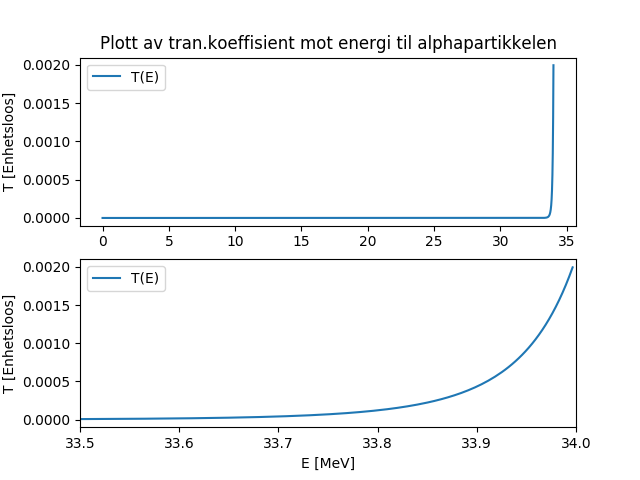
\includegraphics[scale=0.8]{Figur_07.png}
				\begin{flushleft}
Ut i fra plottet fant jeg at $T(4.08) = 7.7 \cdot 10^{-36}$ og at $T(9.85) = 5.9 \cdot 10^{-32}$ og forholdet mellom dette blir $\frac{T(9.85)}{T(4.08)} = \frac{5.9 \cdot 10^{-32}}{7.7 \cdot 10^{-36}} = 7700$. Vi har fra oppgaveheftet at $T_{1/2, 232} = 1.4 \cdot 10^{10} \text{år}$ og $T_{1/2, 218} = 1.0 \cdot 10^{-7} \text{s} = 3.171 \cdot 10^{-15} \text{år}$ og forholdet mellom disse blir $\frac{T_{1/2, 218}}{T_{1/2, 232}} = \frac{3.171 \cdot 10^{-15} \text{år}}{1.4 \cdot 10^{10} \text{år}} = 2.3 \cdot 10^{-25}$. Ser at forholdet her er helt enormt liten, og derfor kan ikke denne transmisjonskoeffisienten forklare den ekstreme forskjellen i halveringstid.
				\end{flushleft}








			\subparagraph{e)}
				\begin{flushleft}
Bruker likningen for transmisjonkoeffisienten for energien $4.8 \text{MeV}$. Bruker samme potensial $V_0 = 34 \text{MeV}$ som tidligere og samme $\Delta x = 17 \text{fm}$. Metoden blir også den samme som i forrige, altså bruker jeg samme masse $m$.
				\end{flushleft}
				\begin{gather*}
T(4.8) = \frac{1}{1 + \frac{34^2}{4 \cdot 4.8 \cdot ( 34 - 4.8 )} \cdot \sinh^2\left( \frac{17 \cdot \sqrt{2 \cdot 3727 \cdot ( 34 - 4.8 )}}{1.973 \cdot 10^{2}} \right)} = 2.35 \cdot 10^{-35}
				\end{gather*}
				\begin{flushleft}
Sannsynligheten for transmisjon er gitt med transmisjonkoeffisienten, altså må partikkelen treffe barrieren ca. $N = 4 \cdot 10^{35}$ ganger for at partikkelen skal ha en god sjanse for å komme ut. Hvis alfa partikkelen har en hastighet på $0.073 c$ så vil partikkelen treffe barrieren etter å ha beveget seg en lengde lik radien til kjernen ganget med to. Unntaket er selvfølgelig første gang, men denne forskjellen i avstand er så liten at vi ikke bryr oss noe om den. Det vil si at tiden er gitt ved $t = \frac{N \cdot 2 \cdot r}{v} = \frac{4 \cdot 10^{35} \cdot 2 \cdot 7.3 \cdot 10^{-15} \text{m}}{0.073 c} = 2.67 \cdot 10^{14} \text{s} \approx 8.5 \cdot 10^{6} \text{år}$ hvis vi tenker klassisk mekanikk, noe vi kan siden vi har en fart mindre en ca. $10 \%$ av $c$. Halveringstiden til radium er $1600 \text{år}$ mens den vi finner ved hjelp av det grove overslaget er åtte og en halv millioner år. Det er en ganske stor forskjell.
				\end{flushleft}









			\subparagraph{f)}
				\begin{flushleft}
Var nødt til å bruke pikometer i steden for femtometer for at programmet skulle fungere. \\
Utslaget ser ut til å bevege seg på en realistisk måte, men verdiene langs $y$-aksen ser ikke ut til å gi noe mening. De virker som de har blitt ganget med $1000$, for når jeg integrerer over en $\Psi(x, t_1)$, der $t_1$ er ett tilfeldig tidspunkt, så får jeg en verdi på ca. $1000$ til sammen, isteden for $1$ som jeg egentlig skulle fått. \\
Bølgefunskjonen beveger seg mot høyre, altså fra negativ til positiv $x$ verdi, helt til den treffer potensialveggen. Da smører den seg opp langs veggen og blir til en veldig høy, tynn, topp. Når den omtrent bare er en høy, tynn, strek vil den begynne å synke ned igjen og bevege seg mot venstre. Nå vil bølgen ikke lenger være en høy bølge med en topp, men heller en breiere en, med flere mindre topper. Det skal også gå en liten bit av bølgen forbi potensialmuren, men det fikk jeg ikke til å visualisere fordi denne biten vil bli alt for liten til at datamaskinen kan registrere. Derimot får jeg et lite utlag inni potensialbarieren, som også er forventet.
Egentlig så burde det jo også vært et potensial på den andre siden av $x = 0$ for å gjøre dette mer realistisk, men siden det ikke gjør det vil bølgen bare fortsette mot venstre.
				\end{flushleft}
\lstinputlisting{Hjemmeeksamen_2f.py}
				\begin{figure}[H]
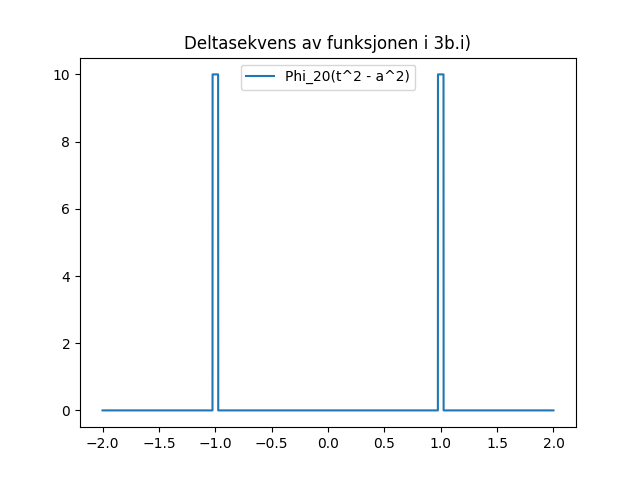
\includegraphics[scale=0.7]{Figur_HE_1.png} \\
\caption{Før bølgen treffer potensialet}
				\end{figure}
				\begin{figure}[H]
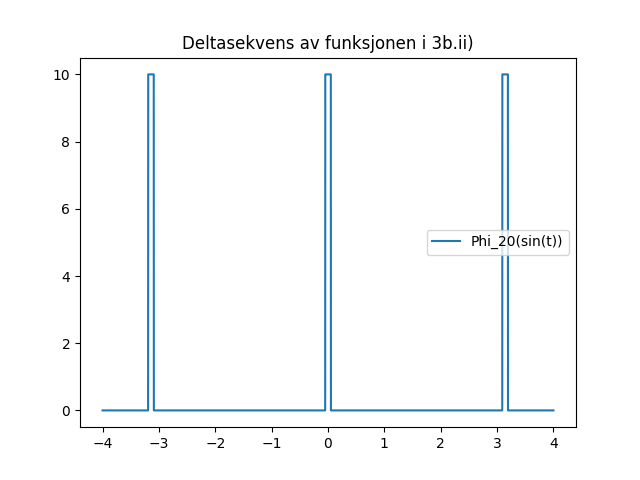
\includegraphics[scale=0.7]{Figur_HE_2.png} \\
\caption{Mens bølgen treffer potensialet}
				\end{figure}
				\begin{figure}[H]
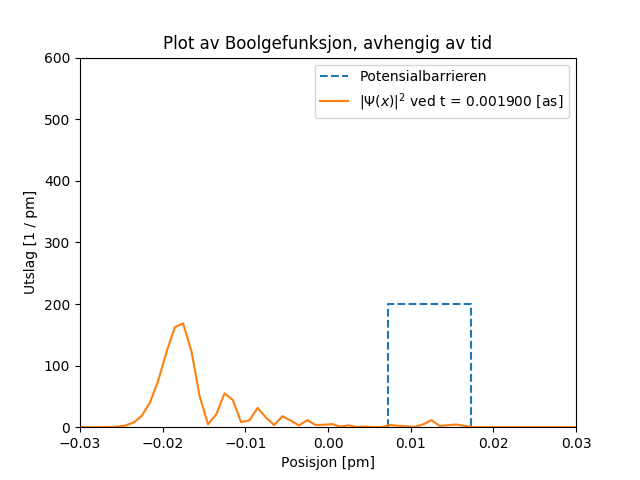
\includegraphics[scale=0.7]{Figur_HE_3.png} \\
\caption{Etter at bølgen har sluttet å reagere med potensialet}
				\end{figure}






			\subparagraph{g)}
				\begin{flushleft}
Forskjellen mellom potensialene er at \textbf{Potensial $1$} er en barriere som er konstant over ett interval, mens \textbf{Potensial $2$} er en barriere som plutselig har en stor verdi, men avtar gradvis hvis bølgen beveger seg lenger til høyre. Det virker mer troverdig at potensialet vil avta gradvis med avstanden fra kjernen istedenfor at det fungerer som en plutselig vegg og stopper veldig brått etterpå. \\
Jeg tipper at transmisjonskoeffisienten vil starte å stige ved en mye tidligere energi, siden det ikke krever så mye energi før litt av bølgen kommer seg igjennom, men at den fortsatt vil ha en veldig bratt økning når energien nærmer seg $E = Z_{\alpha} Z_{D} k_{e}$. \\
Bølgefunksjonen, som funksjon av tid, vil bevege seg til høyre i starten som tidligere, men når den treffer potensialveggen vil en større andel av den gå igjennom enn tidligere. Den vil antageligvis fortsatt smøre seg opp mot veggen, og deretter begynne å gå mot venstre, men nå vil den ende opp med enda lavere topper enn tidligere.
				\end{flushleft}
\end{document}